\documentclass[11pt,a4paper]{book}
\usepackage{algorithm}
\usepackage{algpseudocode}
\usepackage[pdftex]{graphicx}
\usepackage{setspace}
\usepackage{nameref}
\usepackage{amsthm}
\newcommand{\HRule}{\rule{\linewidth}{0.5mm}}
\renewcommand*{\familydefault}{\sfdefault}
\graphicspath{ {graphs/} }

\newtheoremstyle{named}{}{}{\itshape}{}{\bfseries}{.}{.5em}{#1 \thmnote{(#3)}}
\theoremstyle{named}
\newtheorem*{definition}{Definition}

\begin{document}

\doublespacing
\begin{titlepage}
\begin{center}


\includegraphics[width=0.15\textwidth]{./logo}~\\[1cm]

\textsc{\LARGE Indian Institute of Technology, Kanpur}\\[1.5cm]

\textsc{\Large }\\[0.5cm]

% Title
\HRule \\[0.4cm]
{ \huge \bfseries Latency Bound Data Collection from Sparse Sensor Networks Using Data MULEs \\[0.4cm] }

\HRule \\[1.5cm]

% Author and supervisor
\begin{minipage}{0.4\textwidth}
\begin{flushleft} \large
\emph{By:}

Aman Kumar Singh
\end{flushleft}
\end{minipage}
\begin{minipage}{0.4\textwidth}
\begin{flushright} \large
\emph{Supervisors:}

Dr. R. K. Ghosh (IIT Kanpur)

Dr. Maitreya Natu (TRDDC, TCS, Pune)
\end{flushright}
\end{minipage}

\vfill

% Bottom of the page
{\large \today}

\end{center}
\end{titlepage}

\tableofcontents
%\begin{abstract}
The positive effect of multiple mobile data collectors (or Mobile 
Ubiquitous LAN Extensions or MULEs) on network lifetime and energy 
efficiency of a sparse sensor network, when used in data collection from 
them, is well known. However, the increased latency (due to physical 
movement of a robot instead of radio communication) may be a problem in 
some latency sensitive applications. Motivated by this problem, many 
MULE path scheduling problems in attempts to decrese latency 
employ multiple MULEs and long range relay nodes for data collection 
from the sensor network. Most of the work 
use some kind of network partitioning schemes that do not make use of 
rendezvous of two MULEs. To overcome this problem, some of these works 
use long range relay nodes or a common point of origin of the data 
collection tours of all the employed MULEs. In this thesis we 
consider latency bound data collection from a sparse sensor network 
using only MULEs as the means to eatablish connectivity, and also 
alleviate the problems mentioned above. The sensors in the field are 
grouped under planar circular discs of radius equal to their sensing 
range using disc cover problem. The centers of these discs are called 
"location nodes". In other words, locations nodes define the positions
where a MULE comes to gather data from the sensors covered by it. The 
latency bound, given as an input, determines 
the bound on the path length of a MULE. Using this bound, we propose a 
MULE path selection heuristic, which divides the movement and data 
collection work among multiple MULEs, each of whose data collection tour 
respects the bound. The tours are chosen in such a way that the MULEs 
which are supposed to rendezvous for forwarding data, have a definite 
rendezvous point in the plane to do the same.

\end{abstract}
\chapter{Introduction}


Wireless Sensor Networks consist of a large number of sensor nodes, which are battery-powered, low energy consuming devices. Wireless Sensor Networks (WSNs) are used for applications such as monitoring (e.g., pollution prevention~\cite{application2}, structures and buildings health), event detection (e.g. fire hazard ~\cite{application5}) and target tracking (e.g., surveillance~\cite{application3}). These devices perform three basic tasks:
\begin{itemize}
\item Sample a physical quantity from the surrounding environment
\item Process and buffer the acquired data
\item Transfer the data through wireless communications to a data collection point called sink node or base station.
\end{itemize}
The sensors, as soon as deployed on the field, identify their adjacent sensors (neighbours), and are able to form an ad-hoc network. If this network is connected (each sensor is able to send data to another sensor on the field through one or multiple hops), then it is called a dense sensor network. Such a network is used as basic infrastructure for routing sensor-acquired data to the sink node (Base Station) using WSN routing protocols~\cite{routingSurvey}. Occasionally, sink node may send data to all sensor nodes as well. 

However, dense networks are seldom realizable in practice. Usually, sensors are spread (air dropped) over a large geographical area resulting in a sparse network. This kind of networks are useful for applications (e.g., environmental monitoring applications~\cite{sparseEx}) where fine-grained sensing is not required. In sparse sensor networks, islands of sensor sub-networks are formed (WSN islands~\cite{intro2}), which cannot communicate to each other without external help. Data collection from this kind of network, without deploying additional sensors can be done using:
\begin{itemize}
\item Long range relay nodes~\cite{relayNodes}
  
Long range and high power nodes, whose main purpose is to establish connectivity among such WSN islands, and their connectivity to the base station by relaying/receiving data to/from sensors out of range of the local island. Their placement in a sensor network is a well studied problem.
\item Mobile data collectors (MDCs)~\cite{intro3} or Mobile Ubiquitous LAN Extensions (MULEs)~\cite{intro1}: 
  
Controlled mobile robots acting as mobile sinks/Base stations/relay nodes. These can be programmed to tour any set of locations so as to collect data from the sensors at those positions,] and relay the same to base station directly or through another MULE. Since the sensors have to wait for the MULE to arrive in range
\begin{enumerate}
\item Sensors may be required to have a battery powered passive wake-up radio device~\cite{intro4}, which can be triggered by a nearby MULE. MULE will then be able to collect data from the sensor, and forward the collected data 
when it is in proximity of the base station (or another MULE assigned to relay to the base station~\cite{sim2}). %it will forward this collected data.

\item Sensors wake-up and sleep operation can be controlled at the MAC layer~\cite{dutyCycle1} \cite{dutyCycle2}. In this approach, sensors periodically sleep and wakeup to save power. Data transmission occurs only when the MULE is in range, and the sensor is awake.
\end{enumerate}
\end{itemize}

The MULE approach naturally saves energy of the sensors (hence prolongs network lifetime) as sensors communicate over one hop only and do not perform aggregation or forward data of other sensors. However, the main disadvantage is increase in latency of data transfer from sensors to Base station, and some applications ~\cite{application4} are sensitive to it. This is the reason that the studies on the problems of MULE path optimization and job scheduling are abundant \cite{muleSurvey}.

The main contribution of this work is to add to these studies. Usually these works make use of multiple MULEs by partitioning the network into "equal" parts (in terms of TSP tour time of that partition, together with the time taken to collect data from sensors in that partition), and each partition is assigned to a MULE. Our work takes the required latency constraint of the sensor network application as input and computes the number of MULEs required along with their trajectories. We assume MULEs can move freely in the plane of the sensor network, and they have identical, constant speed.

In the chapter ~\nameref{chap:location_nodes}, we first talk about the components of the general problem of data MULE scheduling, and its part that we are concerned with: Path selection. Then we introduce location nodes and the heuristics suggested to compute them. We also show justification of our choice of heuristic with performance measures. In the chapter ~\nameref{chap:steiner}, we describe our main heuristic for path selection and provide pseudocode for it.

The future works chapter contains two directions this work can take, which we can see at the time. First is the addition of obstacle avoidance capability to the algorithm, and the second is the application of another work (on optimization of TSP tours in presence of neighbourhoods) into this work.


\chapter{Preliminaries and Subproblems}
%\label{chap:location_nodes}

\section{Path Selection of Mobile elements}

It is known that controlled MULEs can increase a WSN's lifetime by saving energy. But the problem of planning an optimal path and job schedule is a hard problem in general, known as the Data MULE scheduling problem \cite{dms}. It has three components:
\begin{enumerate}
\item Path selection: which trajectory the data mule follows
\item Speed control: how the data mule changes the speed while moving along the path
\item Job scheduling: from which sensor the data mule collects data at each time point
\end{enumerate}
In this thesis we will focus only on Path selection of the MULEs.

\section{Geometric Disc Covering and Location Nodes}

In the interest of collecting data from sensors in one hop, we propose to cover the sensor field with circular discs of radius equal to the range of the sensors. The centers of these discs are going to be locations where MULEs will pause to collect data from the sensors. We call these positions \emph{location nodes} for convinience. Our path selection heuristic uses location nodes as vertices of a graph embedded on the 2D plane. Ofcourse, we are approximating the communicable region of a sensor to a circular disc, and also assuming that the range of the MULE is greater than that of any sensor (we assume all the sensors are identical in communication range). The centres of these discs are called \emph{location nodes}.

There are many \cite{} \cite{} geometric disc covering heuristics and PTASs, any one of which can be used here. But since PTAS's having high running time \cite{} and hard to implement, we used heuristics for the implementation. Following are some heuristics that we tested on sample fields.

\subsection{Preliminaries}
\label{subsec:prelim}

Let $P$ be the set of points to be covered with discs of radius $R$, in the square field $F$. For any two $p_1, p_2 \in P$, there are two $c_1,c_2 \in F$ (called "crosses" for convinience) such that $p_1$ and $p_2$ will lie at the boundary of a disc of radius $R$ placed at either $c_1$ or $c_2$. We consider points $p_1$ and $p_2$ as covered (barely) by any of the two discs above. For any two points $p_1$ and $p_2$ such that distance between $p_1$ and $p_2$ is less than $2R$, there exist two crosses $c_1$ and $c_2$ ($c_1$ and $c_2$ are said to "involve" $p_1$ and $p_2$ for convinience). Let $C$ be the set of all possible crosses in the field $F$.

A set $S$ of disc centres such that they cover all the points in the field $F$ is called a solution of the MGDC problem in the field $F$. Let $S_1$ be such a solution. Then there exists a solution $S_2 \subset C$ such that $|S_1|=|S_2|$.

\subsection{Heuristics}

\begin{description}

\item[OPT] This is the optimum solution algorithm, which uses brute-force to search for the minimum set cover to find the optimum solution. First we make a table of the information regarding which cross (refer \ref{subsec:prelim} covers which sensors. These crosses act like the subsets of the ste of sensors, containing the sensors they cover. We then find the minimum set cover using brute-force. Needless to say, the running time of this algorithm blows up very fast.

\item[JGRD] This is originally a set cover heuristic \cite{jgreedy}. Consider the set $P$ as the target set to be achieved from the union of smaller subsets, and the discs centered at the crosses in $C$ represent the subsets of points covered by them. Our problem of MGDC then becomes a set cover problem. \cite{jgreedy} gives a greedy heuristic for this.

\item[GRD] (We are not aware of any other work using this heuristic) Let the list of all sensor positions in the field $F$ be $L$. First sort $L$ according to their (x,y) position co-ordinates (first by x co-ordinate and then by y co-ordinate). Starting from the first sensor $p$ in the list, pick the disc which covers maximum number of uncovered sensors and covers $p$ too. To do this, compute all the crosses in $C$ which involve $p$. Place a disc of radius $R$ at each of the crosses, and choose the cross whose disc covers the most number of points. Choose the next uncovered sensor in $L$ and repeat the covering procedure, until all sensors are covered.

\item[SHFT] The shifting strategy from \cite{shifting}. This algorithm takes two input parameters: $l$ (shifting parameter, chosen later) and $D$ (diameter of discs to be used for covering). Let the field be a square of length $W$. First we divide the field into vertical strips of width $l \times D$, as shown in figure \ref{fig:origStrip}. We do disc cover on these vertical strips (explained later) individually (treating them as separate fields. The union of the solutions of all the vertical strips is clearly a solution to the problem. This solution is assigned to $current\_solution$. Now, the whole partition of strips is shifted horizontally, away from the origin, by the amount of $D$ (as shown in figure \ref{fig:shiftStrip}). Again, all the strips are covered with discs (to be explained later how), and the union of the solutions of these shifted vertical strips another solution, assigned to $new\_solution$. If the size of $new\_solution$(the number of discs in the solution) is less than the size of $current\_solution$, the current solution now becomes $new\_solution$. We continue shifting the partition and measuring the solutions thus generated $l-1$ times.

To cover a strip of width $w$, we again apply the shifting strategy. We divide the strip into squares of side $w$ (and maybe a remainder rectangle, in case $W$ leaves a remainder upon dividing with $w$). To cover this sqaure (of size $w \times w$) with discs of diameter D, we use the strategy OPT described above. The shifting of this partition is done by the amount $D$ just like in the original field, and the smallest solution is chosen. The shifting parameter $l$ depends on the time constraint one has regarding the running time of this algorithm. It is chosen in such a way that the problem size in each sqaure (of size $w \times w$) is small enough for the OPT to run in required time constraint.

\begin{figure}[H]

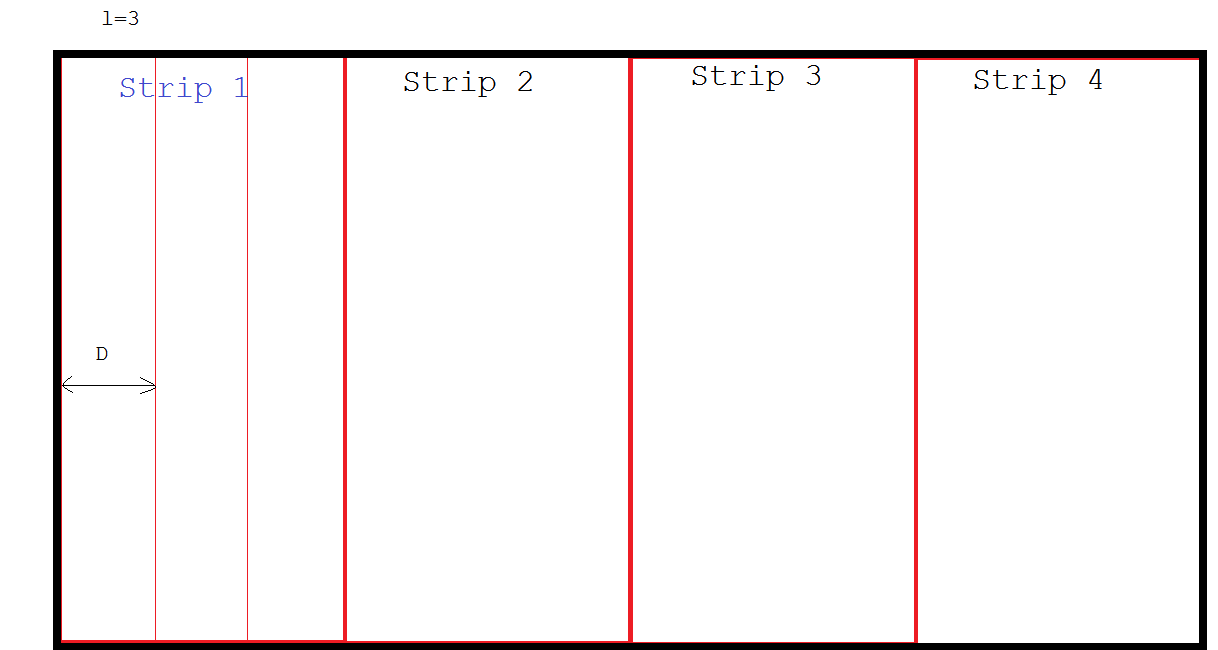
\includegraphics[width=15cm]{figures/beforeShift.png}
\caption{Original division of the field into vertical strips. $l$ is 3 here.} \label{fig:origStrip}

\end{figure}

\begin{figure}[H]

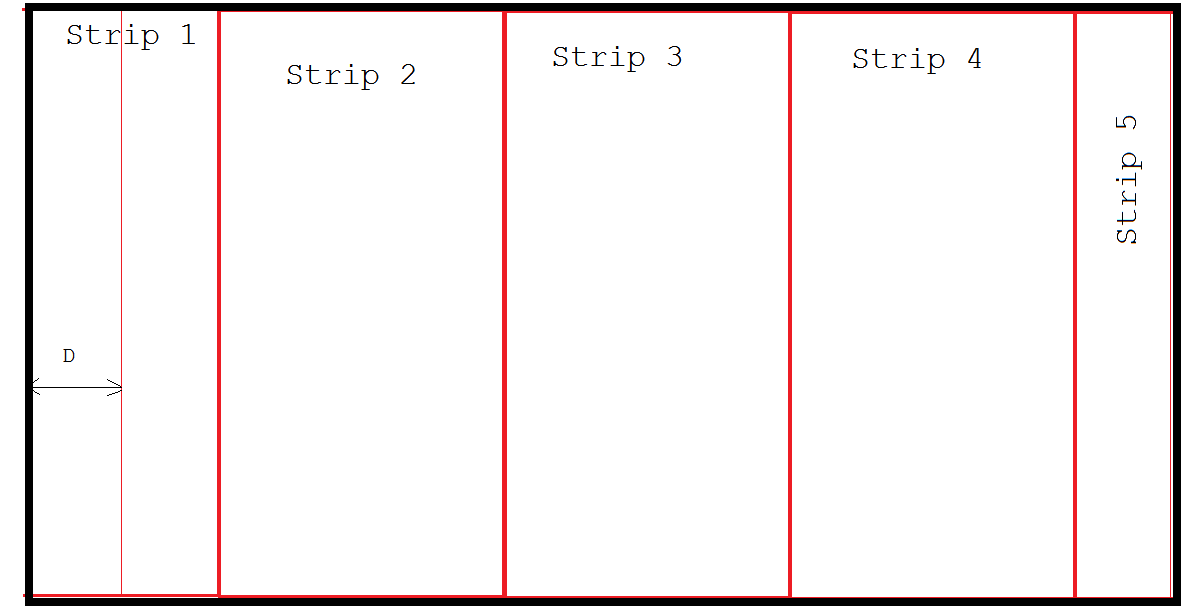
\includegraphics[width=15cm]{figures/afterShift.png}

\caption{After the shift right by the amount $D$}\label{fig:shiftStrip}

\end{figure}

\item[SEL] For any sensor $s$, let $L$ be the set of discs covering it. Pick the disc which covers the least number of sensors.
\item[RND] Randomly pick discs until all the sensors are covered. Just for sake of comparision with other heuristics.
\end{description}

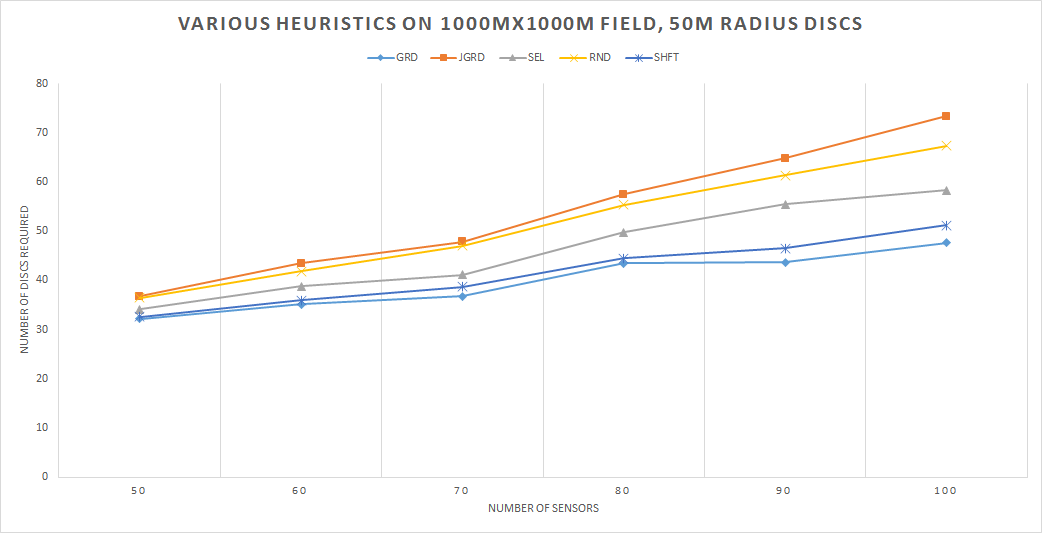
\includegraphics[width=15cm]{discs}
\chapter{Related Works}
Most notable related work is~\cite{sim}. Their goal is to find the trajectories of $k$ MULEs to collect data from the $N$ wireless sensor nodes deployed on 2-D Euclidean space such that the data collection latency (the length of the longest trajectory among k trajectories) is minimized. They consider two cases: 
\begin{description}
\item[Case 1:] Each MULE is connected to the sink only from their original positions (base stations).
\item[Case 2:] Each MULE is connected to the sink directly at any time from any location.
\end{description}
Intuitively, it may be better to utilize MULE to MULE communication too for data transfer, which is absent in their approach but essential to our approach. They solve the problem by formulating $k$-traveling salesperson problem with neighborhood ($k$-TSPN) and $k$-rooted path cover problem with neighborhood (k-PCPN) problems. Their algorithm has a constant factor approximation, however, as they say in section~5 of their paper, this algorithm itself is based on another approximation algorithm~\cite{supportSim}, which is a very complicated rounding-based algorithm and difficult to use. Therefore, they propose heuristics to solve it.

A similar problem of covering a set of points in a plane using multiple robots~\cite{roboPlan} also seemed promising, but, we were unable to accomodate the additional constraints listed above (they use Clique cover problem~\cite{minCliquePartition}, which has its own application in data collection algorithms for dense sensor networks).

Another related work~\cite{sim4} is on SenCars~\cite{sencar} (a MULE). Their algorithm takes as input $m$ the number of SenCars, the sensor network (sensor node positions in the field) and a set of polling points $P$ (positions from where the SenCar can stop and communicate with sensors around it). Their aim is to divide the set of polling points $P$ into subsets $P_1, P_2, \ldots, P_m$, each of which have approximately equal weight. The weight of a subset of polling points is the sum of operation times of a SenCar at each polling point (The time that a SenCar will take to collect data from the sensors covered by that polling point, which is directly proportional to the number of sensors covered by it), plus the time it will take the SenCar to visit each polling point in this partition. They show an integer linear programming formulation of the problem, and also provide a heuristic.

%The greedy heuristic:
%First, MST of polling points made
%w(v) is the weight of the subtree rooted at vertex v.
%We use a variable m to represent the
%number of currently available SenCars in each stage of the algorithm and initialize it to N_k. To build a subtree in each %iteration, first find a farthest leaf vertex v onT with the minimum
%weight. If w(v) < W_T(weight of tree T)/m, find its parent vertex on T, denoted by PA(v), and let v =PA(v). Check its weight %and repeat this up-tracing process until w(v) ≥W_T/m. Record
%this vertex v and consider it as the root of subtreet. All the
%vertices on t will belong to the same part and are removed from
%T, which means that the corresponding selected polling points
%on t will be assigned to the same region (or a SenCar). After
%that, update T, W_T, m and w(v') for each vertex v' on the updated
%T and repeat this operation. When there is only one available
%SenCar left, all the remaining selected polling points and their
%associated sensors are assigned to this SenCar and the procedure terminates.

A drawback in their partitioning approach is that in their TSP evaluation of a partition (the length of tour that the SenCar handling that partition will have to take), the rendezvous of two neighbouring MULEs is not taken in account. In~\cite{sim4}, the authors simply assume that each SenCar can forward the gathered data to one of the nearby SenCars when they move close enough. It is a reasonable assumption in a relatively denser sensor network (where MULEs' tours can be close enough to communicate to each other) because MULEs transfer data at high speed and they aggregate data before transmitting. This facilitates a SenCar to transfer/recieve required data within the brief contact time. But in the case of a sparse sensor network containing sensor islands, each with similar weights, this approach may lead to isolated partitions as the islands may be far away. This will lead to the situation where a SenCar cannot communicate with any other SenCar, because its tour never gets close enough to another SenCar's tour. Our approach ensures connectivity through ensuring MULE rendezvous at some point in the plane.

Reference~\cite{sim3} is a connectivity restoration algorithm for a sparse sensor network. Its authors use both stationary Relay Nodes (RN) and Mobile data collectors, or mobile relay nodes (similar to MULEs) to restore connectivity in a set of sensor islands as their sensor network. They call each island a partition. Although RNs are best for providing stable link from cluster to the sink, there is only a limited number of stationary RNs they can use. For each partition they choose a representative sensor node, which has the responsilbility to collect and store the data from its partition. For these representative nodes, they compute the Steiner tree, for the determination of positions of relay nodes. Since stationary RNs are preferable to MDC's, initially all the relay nodes are mobile (i.e. are MDCs). Each of them visits a subset of representative nodes under bounded latency L. One by one they start connecting each partition to the sink through relay nodes, and at each step they check whether the remaining MDCs are still able to cover the remaining clusters under the bound latency.

Another work that uses Steiner tree to plan MULE path is~\cite{rendezvous}. Their work is applicable only on dense sensor networks, because they use RPs (rendezvous points) situated at steiner points to collect and buffer data from nodes farther away from the bases station for the MULE to visit and collect later. Ofcourse this means they have to be in range of their adjacent snesor in the Steiner tree, which can not be guaranted in a sparse WSN.

\chapter{Path selection} \label{chap:steiner}

%\section{Subproblems}

Our approach to a better heuristic is driven by the concept of location graph and using the same for construction of low latency tours of the MULEs in data collection phase. The two critical subproblems encountered in this context are: 
(i) Euclidean Minimum Stiener Tree (EMST), and (ii)  Euclidean Travelling Saleman Problem (ETSP). The EMST problem has already been introduced in chapter 2. We will briefly restate these here for sake of completeness and convenience in description of our heuristic.

\begin{definition}[Euclidean Travelling Salesman Problem]
Given a set of n 2D points in a plane find a minimum weight length tour of all the points, visiting every point exactly once.
\end{definition}
We use Christofides algorithm~\cite{christofides} as the approximation heuristic for computing TSP route of a set of points.

\begin{definition}[Euclidean minimum Steiner Tree problem]
Given a set $P$ of points in a 2-D plane as input, the output is a network of line segements connecting all of the points in $S$, with the smallest total (Euclidean) length.
\end{definition}
The line segments making the Steiner Tree need just be incident on the points in $S$. This implies that the algorithm is free to use additional points from the plane, if necessary, to produce the smallest total length network. The additional points are called {\em Steiner Points}.

The location nodes (the nodes in location graph) computed earlier, form the set $P$, and the EMST is generated using the set $P$, and is called the location graph $T$. The pseudo code for the heuristic which appear later in section ~\ref{sec:heuristicAlgo} uses the EMST as input. The choice of EMST as data structure over MST is guided by the fact that the weight (weight here means total of lengths of all the edges in a graph) of EMST is always atmost the weight of the MST, and we use the weight of a tree as an approximation of the weight of the TSP tour of its vertices. This leads to needing smaller number of MULEs for achieving same latency bound, as shown in section \ref{sec:compmst}. Furthermore, in the case where the field also includes obstacles, Steiner trees lend themselves naturally to cover all the points due the properties of Steiner points~\cite{oaest99} as explained in section~\ref{sec:steinerPoints} of Chapter~\ref{chapter:2}. Though we plan not to cover the obstacle avoidance case, we briefly sketch the underlying ideas in Chapter~\ref{chap:concl}. 


\section{Path Selection Heuristic}

%\subsection{Aim}
The aim of path selection heuristic is to find a minimum partitioning of
the set of location nodes of a location graph by addition of 
extra Steiner points such that following conditions are satisfied.

\begin{itemize}
\item Each of the subsets has a TSP tour length (in units of time) less than a per-specified value $L$, and for any two sets $S_{i}$ and $S_{j}$, $S_{i} \cap S_{j} \le 1$.
\item Let $V$ be the set of all subsets $S_{i}$. Let $E$ be the set of pairs of subsets $(S_{i},S_{j})$ such that $S_{i} \cap S_{j} = 1$. Then the graph $G(V,E)$ should be a connected graph.
\end{itemize}

It assumed that the time a MULE spends in a network while collecting data
consists of three main components: (i) travelling from one location node to another $t_{TSP}$ (ii) Talking to sensors belonging to a location node $t_{LS}$, called MULE's pause time, at a location node (iii) Talking to other MULEs/Base station $t_{MBS}$.

We assume that MULE to MULE data transfer times are shorterdue to two reasons, namely, (i) MULEs may use data aggregation while sending data to fellow a MULE or BS, and (ii) MULEs being relative expensive and more robust than sensor node, typically have higher bandwidth for inter MULE data transfer. This is the reason, we ignore the contribution of $t_{MBS}$. The component $t_{LS}$ for each location node can be given as an input (observed before running the heuristic, by simply sending one MULE on a tour of all the location nodes in the field to measure and record such times beforehand), or computed using sensor parameters, such as: Sensor data throughput ($SDT$, effective data rate, after taking into account the overhead introduced due to protocol headers) and Sensor data sampling rate ($SSR$, data sampling rate of the sensor, the speed of data acquisition of the sensor from its environment in bytes/sec).


\subsection{Heuristic}

The overall strategy is to create an EMST of the location nodes and then divide this tree into subgraphs, using the tree edges as the guide. Each subgraph's set of nodes will be covered by one MULE (henceforth, this set of nodes will be called a subtour). The term "weight" is equivalent to "time interval" in this algorithm, and is measured in seconds. An edge of the tree is said to have weight equal to its length divided by the speed of the MULE (time taken by the MULE to cover that edge). The weight of a location node is equal to the time a MULE has to wait there for data collection (called pause time). It depends on the latency bound and the number of sensor nodes covered by that location node. Steiner points have zero weight. The weight of the TSP tour of a set of nodes is equal to the smallest amount of time it tales for a travelling salesman to visit each node exactly once.

Consider any euclidean spanning tree of a set of 2D points in a plane (none of the points have any weight). Clearly, one way to visit all points would be to start from the root, and visit the nodes in the depth first search order, always travelling along the edges. This would take time equal to twise the weight of the tree (each edge travelled twice, once for going from parent to child, and once for coming back to the parent from the child). Thus, the optimal travelling salesman tour must be bounded by twice the weight of the tree. 

Now consider the case, when the points have weights too (i.e. the travelling salesman has to wait at the point for a time equal to its weight). Then, the TSP approximation needs to be modified just by adding the total weight of all points in the tree.

Given any tree $T$, we start from the given root node $root$. $root$ then becomes the current node $curr$. Then following steps of Prim's algorithm~\cite{Prim57}, we first mark $curr$ as visited, then we insert all the incident edges of the current node with unvisited nodes to the min-heap $edgeHeap$. Computation of a tour for a MULE consists of two stages coded in two inner while loops.



{\bf Note:} Since we use a 3/2 approximation algorithm \cite{christofides} for computing the TSP tour of a subtour, the bound that we will use in the implementation will be actually $3\times $ weight of the tree. In general, if an $x$ approximation algorithm for euclidean TSP is used, then the bound for TSP weight used should be $2\times x \times$ weight of the tree.

Now we describe the algorithm. Let $boundary$ be a set of nodes of the steiner tree, initially containing any one node from the Steiner tree. The algorithm picks any one node from the $boundary$ and calls it $root$. The algorithm then computes a connected subgraph of the Steiner tree (containing that root node) with bounded TSP time. The nodes of this subgraph form a subtour, covered by one MULE. The boundary nodes of a subgraph are those nodes of the steiner tree (regardless of whether they are location nodes or Steiner points), which belong to the subgraph, and do not have all their adjacent nodes in the subgraph. All the boundary nodes from this subgraph are inserted into $boundary$, and the algorithm is called again. This continues until all the nodes are part of exactly one subtour.

\subsubsection{Preliminaries}

Some data structures and inputs used in the pseudocode are as follows. $T$ is the Steiner tree of the location nodes, given as input to the algorithm. $ASP$ is the average sensor pause time, calculated using $L$ (latency bound), $SDT$ (sensor data throughput) and $SSR$ (sensor data sampling rate). These three are given as input to the algorithm. The map $w$, taken as input by the algorithm, is the map from the nodes in the Steiner tree T to the number of sensors they cover. Each location nodes will have a non zero entry in the map $w$, whereas all the Steiner points will have zero entry in the map. For instance, for a node $v$, $w[v]$ is the number of sensors covered by $v$. $edgeHeap$ is a min-heap of the pairs $(tWeight,edge)$, where $edge$ is a pair of nodes $(v_1,v_2)$, and $tWeight = 3 \times weight\_of\_edge(v_1,v_2) + ASP \times w[v_1]$. The ordering in the min-heap is according to its first argument $tWeight$. To push an edge into the heap $edgeHeap$ means to calculate the $tWeight$ of the edge, then inserting the pair $(tWeight,edge)$ in the heap.

\subsubsection{Computation of subtours}

Computation of subtours begins from the picking of a node form the set $boundary$. This node will be called $root$ for this subtour. Before the computation of the subtour, we mark $root$ as visited, and for all nodes $v$ adjacent to $root$, we push the edges $(v,root)$ into $edgeHeap$.

The subtour is computed in two stages. In the first stage, represented by the first inner while loop, $currSet$ contains the nodes currently included in the subtour being computed. $currT$ is the upper bound of the TSP tour of the nodes in $currSet$; it is updated every time we insert a node into $currSet$. Before popping a pair $(tWeight,edge)$ from $edgeHeap$, we first check for the condition, whether $currT+tWeight$ is greater than $L$; if it is, first stage ends here, and we break from the while loop. Otherwise, we pop the pair $(tWeight,(v1,v2))$ from $edgeHeap$, all the edges incident to $v1$ which have unvisited end nodes are inserted into the heap, $v1$ is inserted to $currSet$, and $currT+=tWeight$.

We keep popping edges from $edgeHeap$ until either $edgeHeap$ becomes empty or, adding any more nodes to $currSet$, leads to $currT$, our current estimate of the weight of the TSP tour of $currSet$, becoming greater than $L$, our given latency bound.  By this time, we are sure that the TSP tour of the nodes in $currSet$ will not exceed $L$.

Observe that any Steiner point whose all adjacent nodes belong to same subtour is useless. Because, such a Steiner point neither serves as a connecting node between different subtours, nor represents a location node. So, such a Steiner point should be eliminated form the subtour. The function $cleanTour$ is used on $currT$ for this purpose, and the first stage ends here.

In the beginning of the second stage, although we are sure that the TSP tour of the nodes in $currSet$ will not exceed $L$, but the actual weight of the TSP tour of the nodes in $currSet$ might be low enough to add still more nodes into $currSet$. For testing whether this is possible or not, first we compute the actual weight of the TSP tour of $currSet$. Then, before adding a node to $currSet$, we test whether its inclusion will make $currT$ exceed $L$ or not. If yes, then $currSet$ is the final subtour for this MULE. Otherwise, the second stage repeats. %until hen our $currSet$ for this MULE is final. 

The edge records still left in the Heap, after completion of one full iteration of the second inner while loop, form the boundary of the nodes in $currSet$. These nodes are pushed in the $boundary$, from where the next $root$ for the next MULE's subtour computation is chosen.% point set to cover, 

\subsubsection{Pseudocode}
\label{sec:heuristicAlgo}

\begin{algorithm}
\caption{Dividing the set nodes with weights of a given Steiner tree into subsets of bounded TSP time}\label{euclid}
\begin{algorithmic}
\Function{greedySteiner}{A Steiner tree $T$ of location in a plane, An array $w$ of the number of sensors under a location node, Starting vertex $root$, desired upper bound on latency $L$}\Comment{this function returns S: Set of tours, each with touring time $\le$ L}
\State Set  $S$
\State $N \gets$ number of vertices in T
\State $hApprox \gets 3.0$
\State $MSPEED \gets$ speed of the MULE used
\State $SDT \gets$ sensor data throughput
\State $SSR \gets$ sensor data sampling rate
\State $ASP \gets$ $\frac{(L\times SSR)}{SDT}$ (average sensor pause time for one sensor)
\State $queue$ boundary.push($root$) 
\State $bool$ $visited[N]$
\State $vertex$ curr 

\algstore{pag}
\end{algorithmic}
\end{algorithm}

\begin{algorithm}
\begin{algorithmic}
\algrestore{pag}

\For{$i \gets 1,N$}
	\State $visited[i] \gets false$ 
\EndFor

\While{1}
	\If{boundary.empty()}
		\State break
	\EndIf
	\State $currT \gets 0.0$ 
	\State $cycleWeight \gets 0.0$ 
	\State Min\_heap $edgeHeap$  
	\State $curr \gets root$ 
	\State Set $currSet$, $tempSet$ 
	\State $visited[curr] \gets true$ 
	\State Set $U \gets$ all unvisited vertices adjacent to $cur$ 
	\ForAll{ vertex $v$ in U}
		\State $edgeHeap.push((hApprox \times dist(v,curr)) + (ASP\times w[curr]) , (v,curr))$ 
	\EndFor

	\State $currSet$.insert($curr$) 
	\While{$\neg$ edgeHeap.empty()}
		\State $nextWeight \gets edgeHeap$.top().first 
		\State $currT \gets currT + nextWeight$ 
		\If{$currT \geq hApprox \times L$}
			break 
		\EndIf
		\State $curr \gets edgeHeap$.top().second.first 
		\State $currSet.insert(curr)$ 
		\State $visited[curr] \gets true$ 
		\State $edgeHeap$.pop() 
		\State $U$.clear() 
		\State $U \gets$ all unvisited vertices adjacent to $cur$ 
		\ForAll{ vertex $v$ in $U$}
			\State $edgeHeap.push((hApprox \times dist(v,curr)) + (ASP\times w[curr]) , (v,curr))$ 
		\EndFor
	\EndWhile

	\State $cleanTour(currSet)$
	
	\State Tour $currTour$ 
	\State $tempSet \gets currSet$ 
	\State $cycleWeight , currTour \gets TSPCircuit(tempSet)$
	\ForAll{ sensor $s$ in $currTour$}
		$cycleWeight \gets cycleWeight + ASP*w[s]$
	\EndFor
	
	\While{$\neg$ edgeHeap.empty() and cycleWeight $<$ $L$}
		\State $curr \gets edgeHeap$.top().second.first 
		\State tempSet.insert(curr);
		\State $cleanTour(tempSet)$
		\State $cycleWeight, currTour \gets TSPCircuit(tempSet)$ 

\algstore{pag1}
\end{algorithmic}
\end{algorithm}

\begin{algorithm}
\begin{algorithmic}
\algrestore{pag1}

		\ForAll{ sensor $s$ in $currTour$}
			$cycleWeight \gets cycleWeight + ASP*w[s]$
		\EndFor
		\If{$cycleWeight$ $>$ $L$}
			\State break 
		\EndIf
		\State currSet.insert($curr$);
		\State $visited[curr] \gets true$ 
		\State edgeHeap.pop() 
		\State $U$.clear() 
		\State $U  \gets$ all unvisited vertices adjacent to $cur$ 
		\ForAll{ vertex $v$ in U}
			\State $edgeHeap.push((hApprox \times dist(v,curr)) + (ASP\times w[curr]) , (v,curr))$ 
		\EndFor
	\EndWhile
	
	\State $S$.insert($currTour$) 

	\While{$\neg$ heap.empty()}
		\State $edge$ $e$ = $edgeHeap$.top().second;
		\State $boundary$.push($e$.second);
		\State $edgeHeap$.pop();
	\EndWhile
	
	\If{$boundary$.empty()}
		\State return false 
	\EndIf

\EndWhile
\EndFunction

\Function{cleanTour}{$vSet$ : the set of vertices in the current tour}
	\Comment{Delete all Steiner vertices from $vSet$, whose all adjacent verices are in $vSet$ itself.}
\EndFunction

\end{algorithmic}
\end{algorithm}

\pagebreak

%\subsection{Scalability restriction and Minimum Latency}
%Consider the extreme case of low latency requirement, when 1 MULE is assigned to each edge of the Steiner tree. This must %be the smallest latency supportable with this heuristic. Lets call this latency $L_{min}$. Let$(i,j)$ be the maximum weighted %edge of the Steiner tree with weight $w_{max}$. Now, suppose for any edge $(p,q)$ in the current Steiner tree, upon %recording the dfs (depth first search) sequence from the base station in the Steiner tree, $p$ appears before $q$; then define %$p$ to be the "near node", and $q$ to be the "far node". Then, in the case of the edge $(i,j)$, say, j being the far node, %$L_{min} \ge w_{max}+t_{LS}[j]$.
%
%Consider a single MULE collecting and aggregating all the data from all the sensor networks, and uploading it to the base %station. For any sensor distribution, let the time taken by the MULE to upload the data be $T_{MBS}$. Now we will account %for $t_{MBS}$. Consider the subtour containing the base station. The MULE assigned to this subtour is responsible for %indirectly collecting and aggregating the data from all other subtours and delivering it to the base station. For this, it %sends/recieves from other MULEs and the base station for total of $2 \times T_{MBS}$ units of time (simplistic assumption, %neglecting time spent in P2P protocol between MULEs). Clearly, for any other subtour, its assigned MULE can not have a %$t_{MBS}$ greater than $2 \times T_{MBS}$. So, if $T_{MBS}$ is significant contribution to total time taken by a MULE to %cover its subtour, $L_{min} \ge w_{max}+t_{LS}[j]+2 \times T_{MBS}$.

\chapter{Results and Conclusions}\label{chapter:5}

%\section{Experiment setup}

We use~\cite{terada} for sensor specification. The sensors are ZigBee temperature sensors, collecting data at one reading per second. In~\cite{terada}, the authors have used 12~bits for one temperature reading. Therefore, our $SSR$ (sensor data sampling rate) is expected to be 1.25 byte/second. The $SDT$ (sensor data throughput) is taken to be 13.4 kbps~\cite{zigbee}. The MULEs' speed is taken to be 10m/s~\cite{muleSpeed}. The sensor positions are chosen randomly in a field of 1000m~$\times$~1000m, and the sensor range is 50m. Note that Zigbee sensor ranges can lie between 10m to 100m.

\section{Simulation results}
\label{sec:sim}
We now present simulation results of our heuristic applied on the following 6 cases:
\begin{itemize}
\item Field size: All Cases: 1000m $\times$ 1000m
\item Sensor Range: All cases: 50 m
\item Number of sensors: Case 1: 50, Case 2: 60, Case 3: 70, Case 4: 80, Case 5: 90, Case 6: 100
\end{itemize}

For each of the above cases we generate 6 random distributions of the sensors, and apply our heuristic on each of them with latency bound of 100 seconds, increasing in steps of 100s until only one MULE is adequate to cover the whole field. The graph "Number of MULEs required vs Required latency bound" for a case is the plot of required latency bound in X-axis, versus, average number of MULEs required to satisfy the latency bound in that case across its 6 random distributions, in Y-axis. The graph "Average latency achieved vs Number of MULEs employed" for a case is the plot of number of MULEs employed in the case in X-axis, versus, the average latency achieved by these many MULEs in this case, across the 6 random distributions.

Each of the following subsections contain results for the respective cases.

\subsection{50 sensors}

\begin{figure}[H]
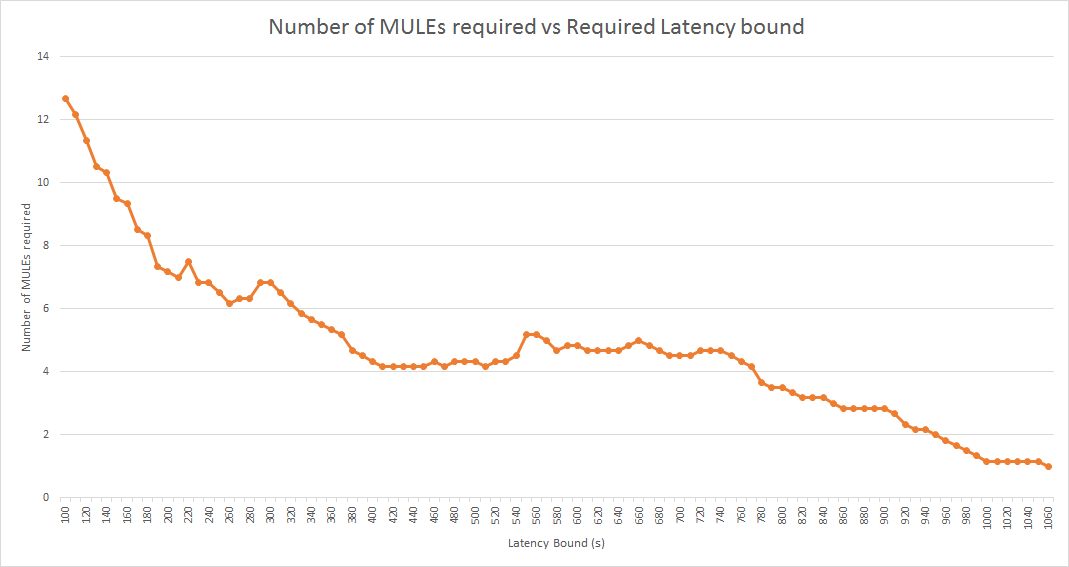
\includegraphics[width=15cm]{50/res_avg.png}
\label{fig:avg50}
\caption{Number of MULEs required vs Required latency bound for 50 sensors}
\end{figure}
\begin{figure}[H]
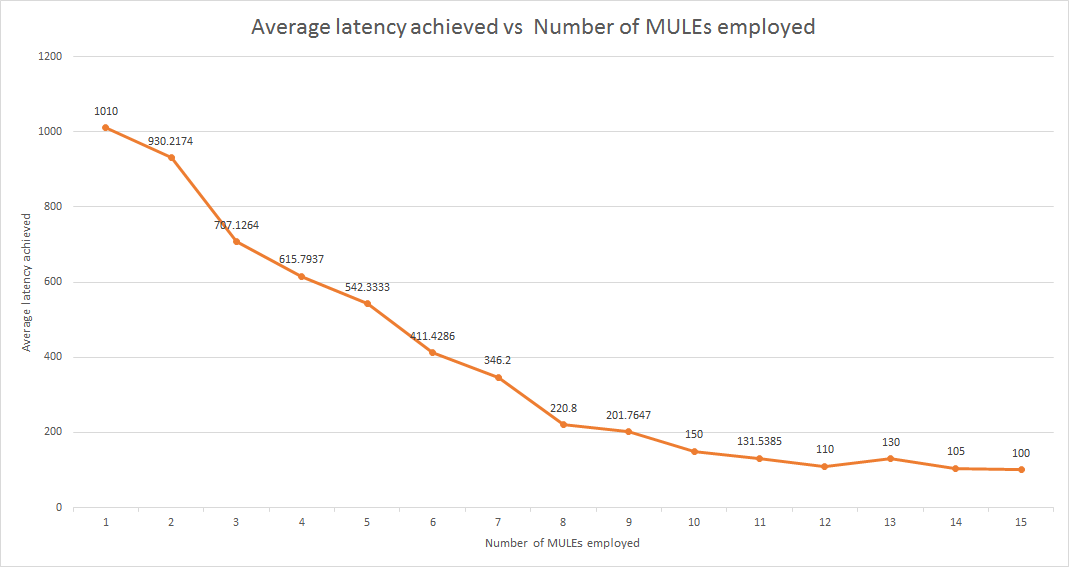
\includegraphics[width=15cm]{50/res_lat.png}
\label{fig:lat50}
\caption{Average latency achieved vs Number of MULEs employed for 50 sensors}
\end{figure}

\subsection{60 sensors}

\begin{figure}[H]
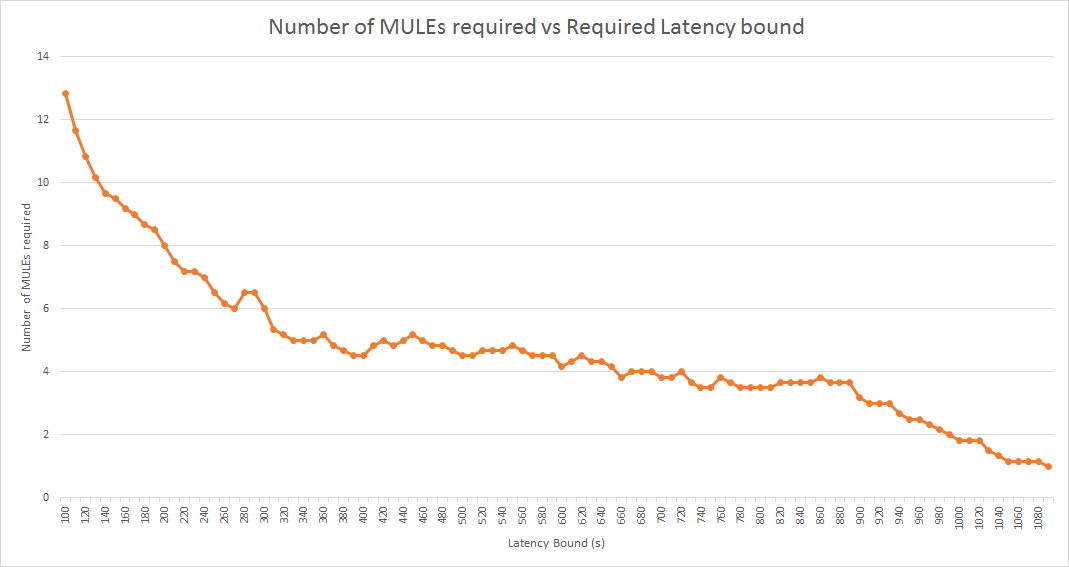
\includegraphics[width=15cm]{60/res_avg.png}
\label{fig:avg60}
\caption{Number of MULEs required vs Required latency bound for 60 sensors}
\end{figure}
\begin{figure}[H]
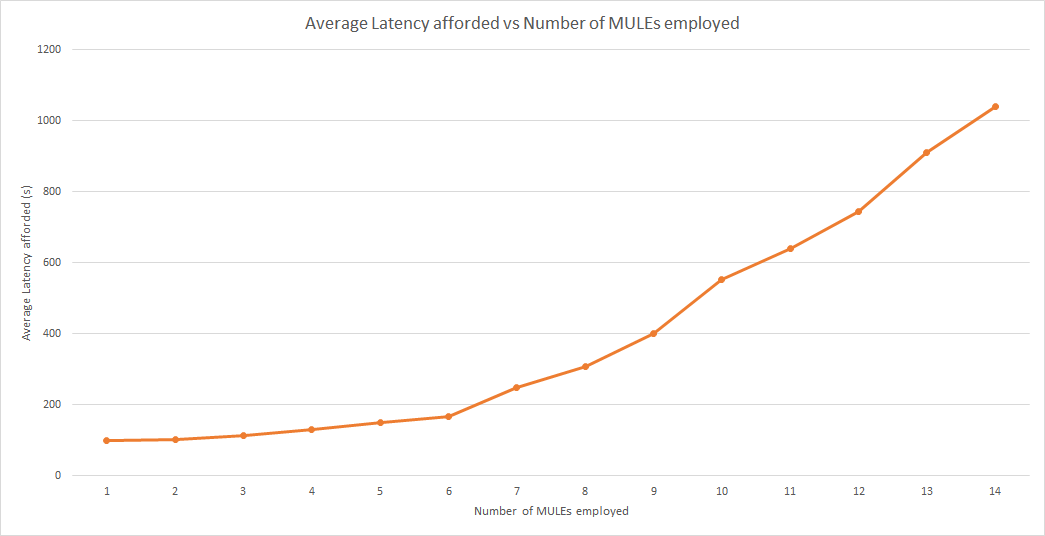
\includegraphics[width=15cm]{60/res_lat.png}
\label{fig:lat60}
\caption{Average latency achieved vs Number of MULEs employed for 60 sensors}
\end{figure}

\subsection{70 sensors}

\begin{figure}[H]
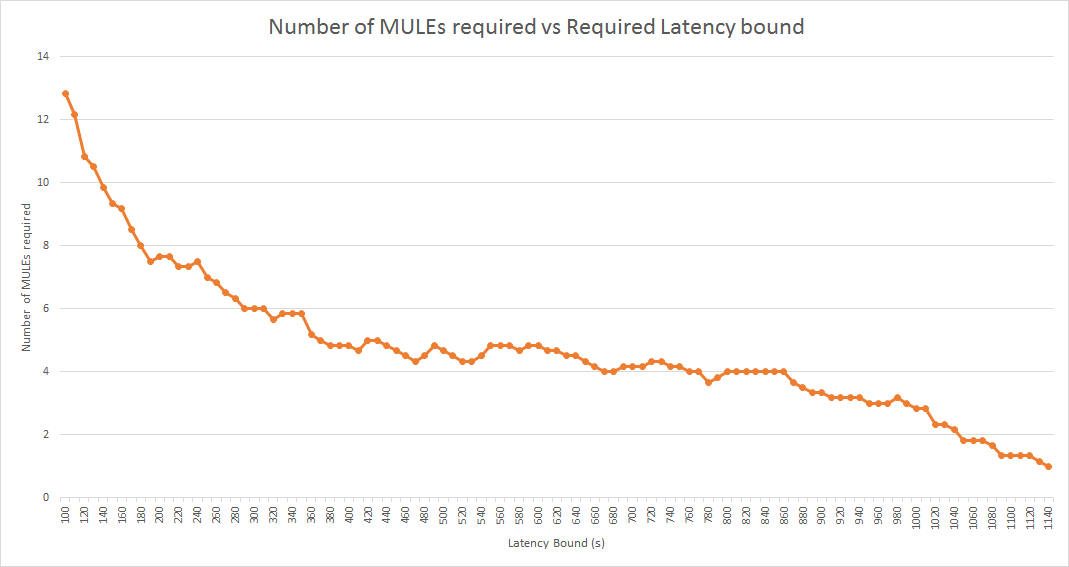
\includegraphics[width=15cm]{70/res_avg.png}
\label{fig:avg70}
\caption{Number of MULEs required vs Required latency bound for 70 sensors}
\end{figure}
\begin{figure}[H]
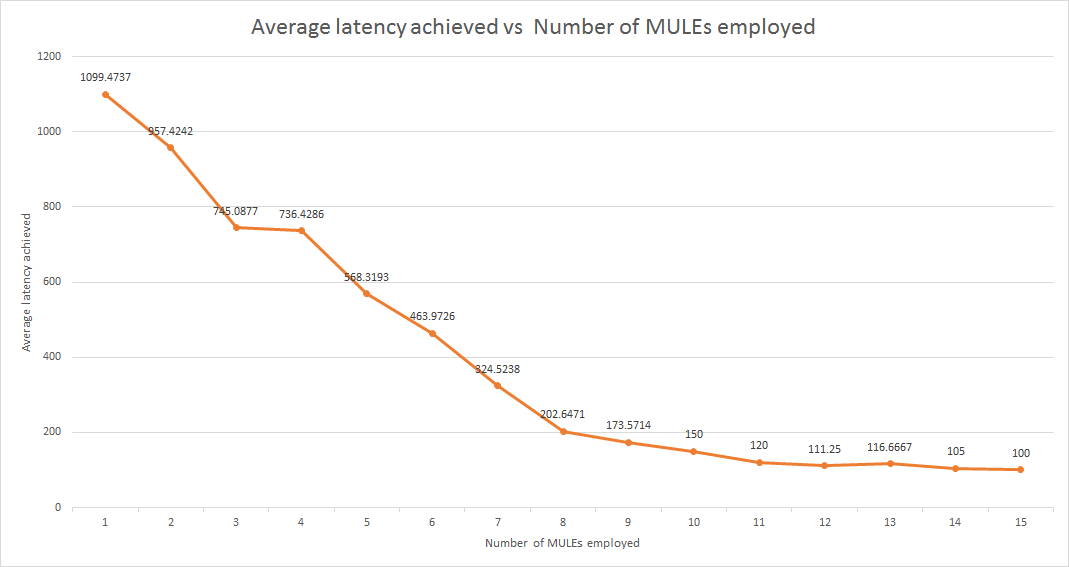
\includegraphics[width=15cm]{70/res_lat.png}
\label{fig:lat70}
\caption{Average latency achieved vs Number of MULEs employed for 70 sensors}
\end{figure}

\subsection{80 sensors}

\begin{figure}[H]
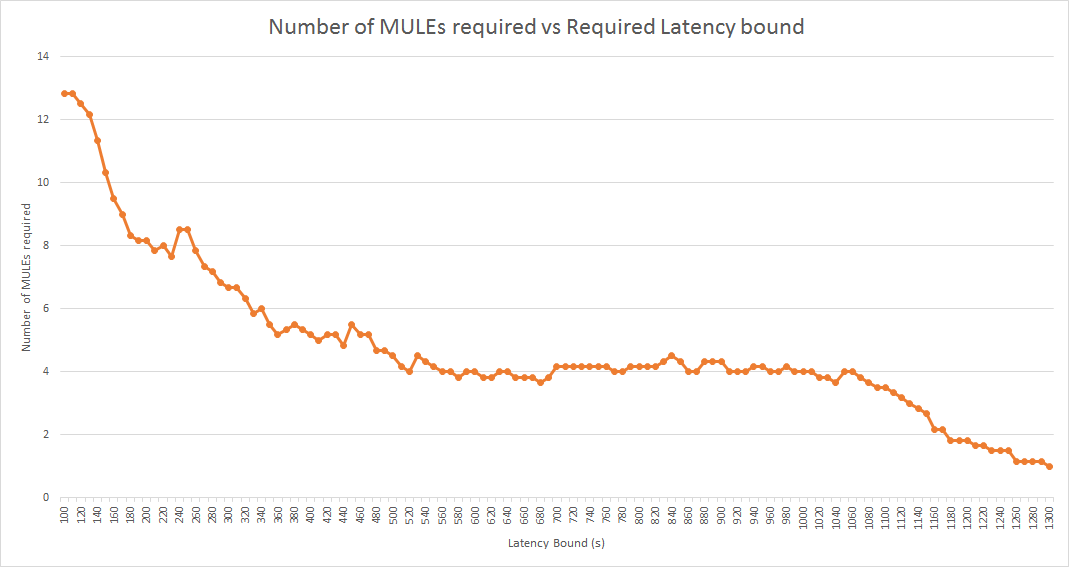
\includegraphics[width=15cm]{80/res_avg.png}
\label{fig:avg80}
\caption{Number of MULEs required vs Required latency bound for 80 sensors}
\end{figure}
\begin{figure}[H]
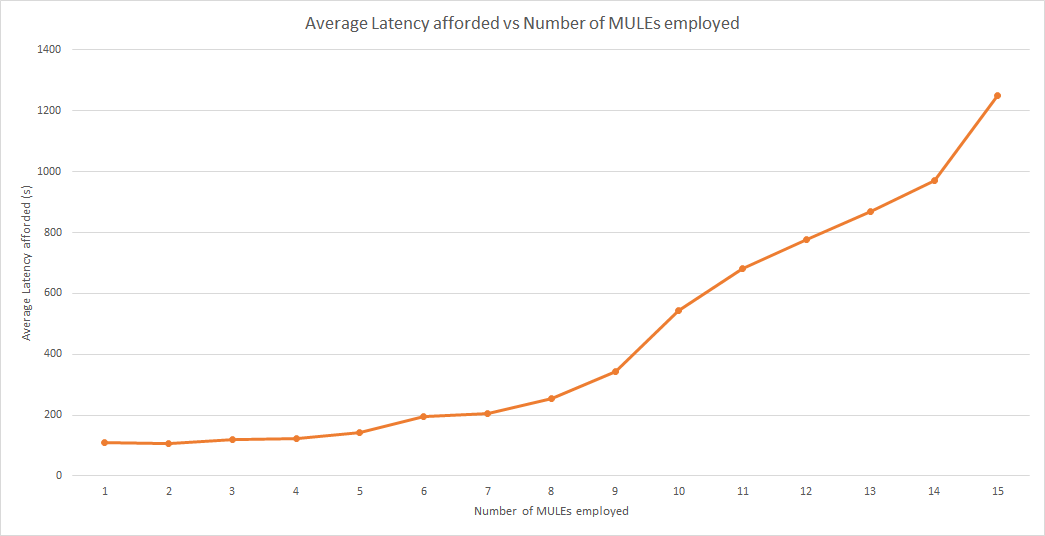
\includegraphics[width=15cm]{80/res_lat.png}
\label{fig:lat80}
\caption{Average latency achieved vs Number of MULEs employed for 80 sensors}
\end{figure}

\subsection{90 sensors}

\begin{figure}[H]
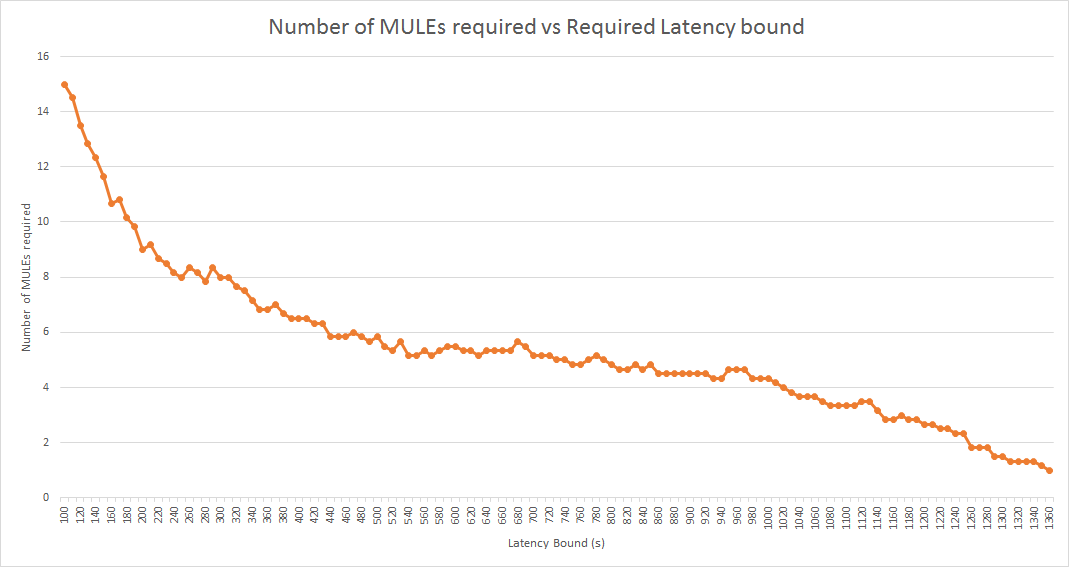
\includegraphics[width=15cm]{90/res_avg.png}
\label{fig:avg90}
\caption{Number of MULEs required vs Required latency bound for 90 sensors}
\end{figure}
\begin{figure}[H]
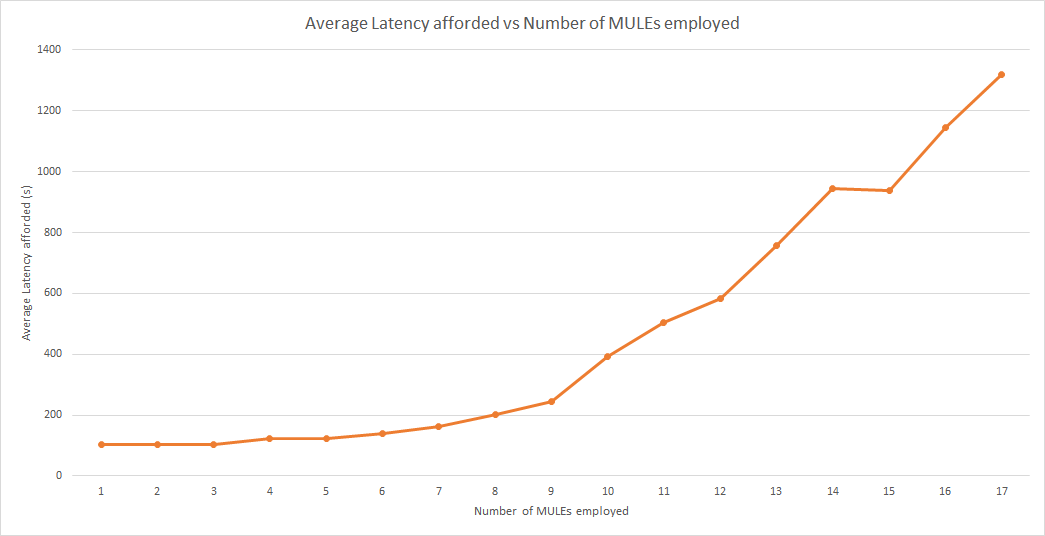
\includegraphics[width=15cm]{90/res_lat.png}
\label{fig:lat90}
\caption{Average latency achieved vs Number of MULEs employed for 90 sensors}
\end{figure}

\subsection{100 sensors}

\begin{figure}[H]
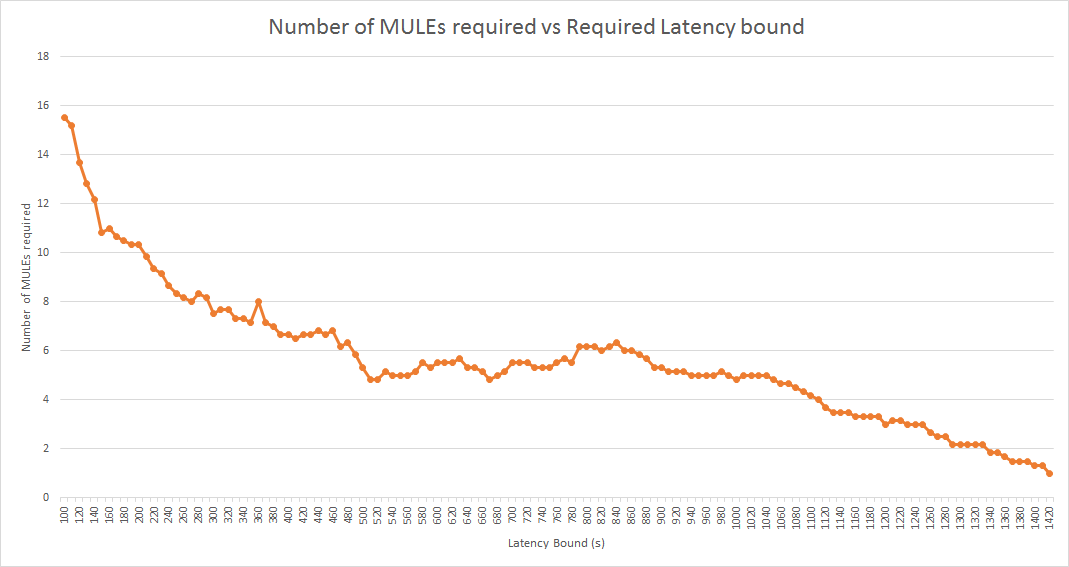
\includegraphics[width=15cm]{100/res_avg.png}
\label{fig:avg100}
\caption{Number of MULEs required vs Required latency bound for 100 sensors}
\end{figure}
\begin{figure}[H]
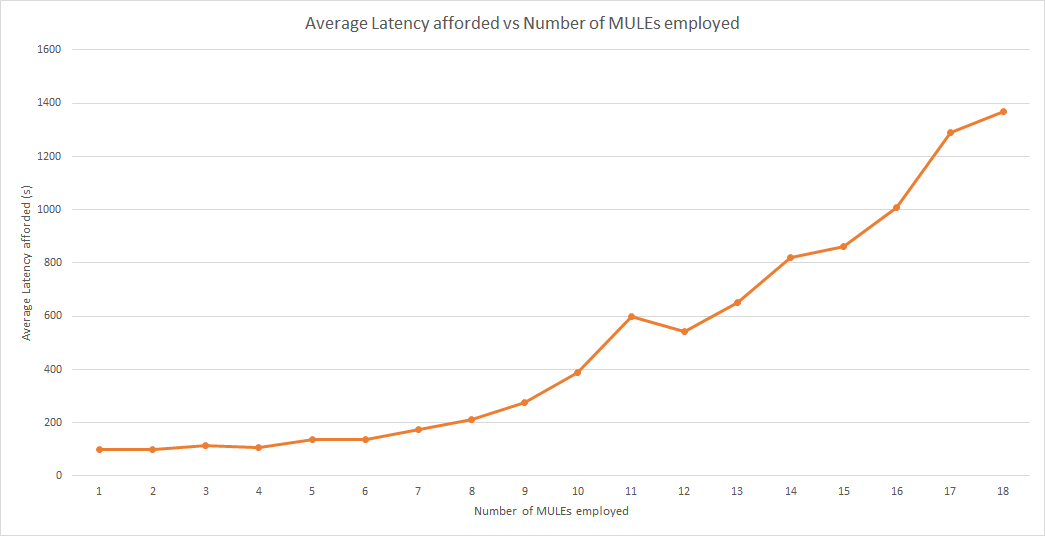
\includegraphics[width=15cm]{100/res_lat.png}
\label{fig:lat100}
\caption{Average latency achieved vs Number of MULEs employed for 100 sensors}
\end{figure}

\subsection{Overlapping plot for 50, 80 and 100 sensors}

\begin{figure}[H]
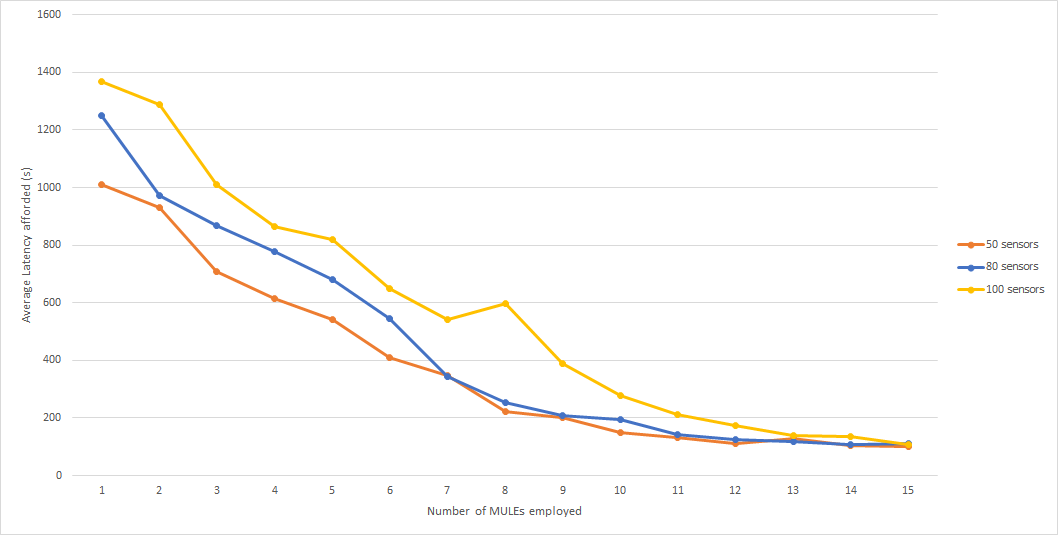
\includegraphics[width=15cm]{figures/latComp.png}
\label{fig:latov}
\caption{Overlapping plot of Average latency achieved vs Number of MULEs employed for 50, 80 and 100 sensors}
\end{figure}

\pagebreak

\section{Comparision of performance with Minimum Spanning Trees}
\label{compmst}

To support our claim in chapter \ref{chap:steiner} that Steiner trees are better suited for network formation of location nodes than MSTs, we applied our heuristic to MSTs of location nodes instead of Steiner trees, and compared their Average latency achieved vs Number of MULEs employed for the cases of 50, 80 and 100 sensors, with their Steiner tree counterparts, as presented below.

\begin{figure}[H]
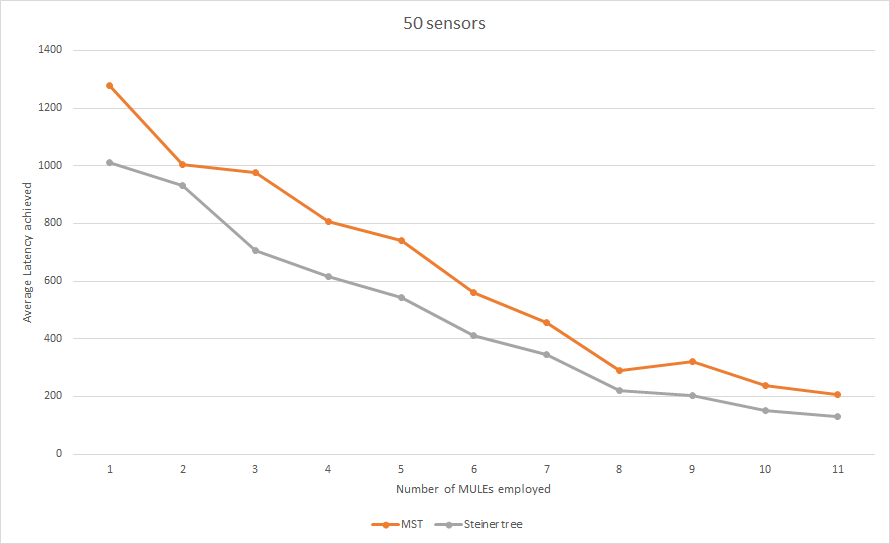
\includegraphics[width=14cm]{steiner_vs_mst/50.png}
\caption{Average latency achieved vs Number of MULEs employed for 50 sensors}
\end{figure}

\begin{figure}[H]
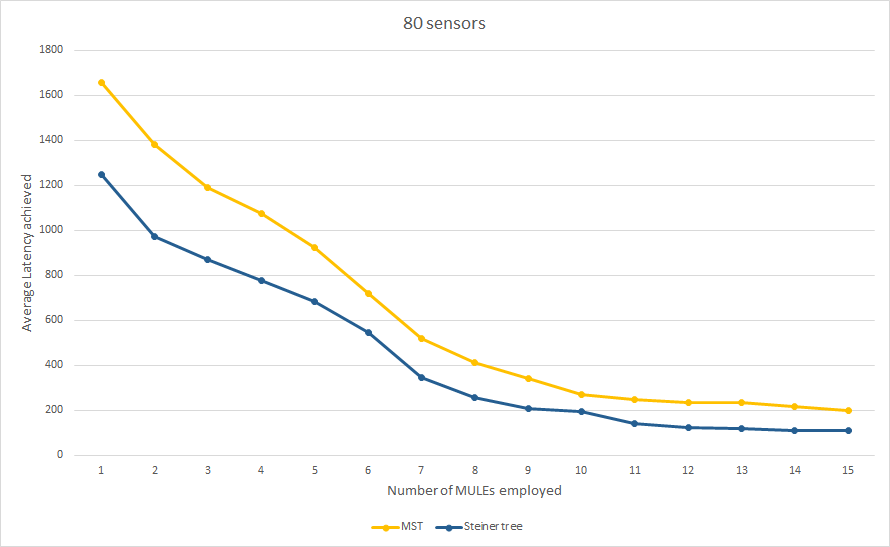
\includegraphics[width=14cm]{steiner_vs_mst/80.png}
\caption{Average latency achieved vs Number of MULEs employed for 80 sensors}
\end{figure}

\begin{figure}[H]
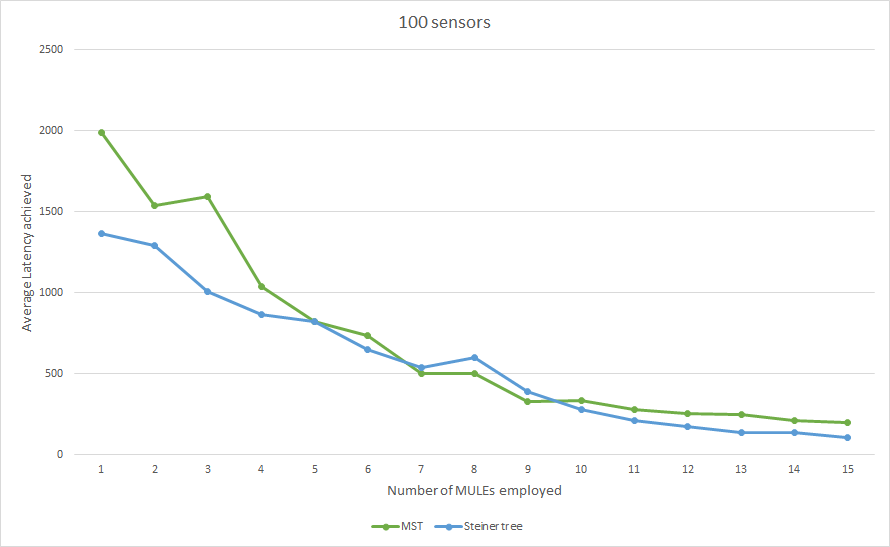
\includegraphics[width=14cm]{steiner_vs_mst/100.png}
\caption{Average latency achieved vs Number of MULEs employed for 100 sensors}
\end{figure}


\section{Conclusions}

As we can see from the "Number of MULEs required vs Required latency bound" graphs of each case from the section \ref{sec:sim}, the decrease in number of MULEs required to fulfill the required latency bound, is not uniform with respect to the increase in the latency bound. For instance, in 70 sensors case, for an increase of latency bound from 100 seconds to 290 seconds decreases the number of MULEs required from 13 to 6. However, for further drop in number of MULEs from 6 to 1, the increase in latency bound is from 290 seconds to 1140 seconds. Similarly, from the "Average latency achieved vs Number of MULEs employed" graphs of each case, we can observe that the decrease in the affordable latency bound is not uniform with respect to the increase in the number of MULEs employed. E.g in 70 sensors case (figure \ref{fig:lat70}), increasing the number of MULEs from 1 to 8 causes the affordable latency to drop from 1100 seconds to 202 seconds. But, a further increase of 7 MULEs decreases the latency only to 100 seconds. 

Therefore, we can conclude that the relation between latency bound and the number of MULEs required is not linear, and after a certain number of MULEs employed, additional MULEs do not achieve significant latency decrease. Let us call this number of MULEs a "flat point" for convinience of reference. Also, let the number of MULEs to achieve latency of 100 seconds in a case be called its "max point". The existence of flat points should be apparent from the table \ref{table:flat}. In the table, $\delta f$ denotes decrease in latency from 1 MULE to flat point and $\delta m$ is decrease in latency from flat point to max point.

\begin{table}
\centering
\caption{Table of flat points in sample sensor node fields} \label{table:flat}
 \begin{tabular}{||c c c c c||}
 \hline
 Number of sensors & max point & flat point & $\delta f$ & $\delta m$ \\  
 \hline\hline
 50 & 15 & 8 & 790 s & 120 s\\ 
 \hline
 60 & 14 & 9 & 872 s & 68 s\\
 \hline
 70 & 15 & 8 & 897 s & 102 s\\
 \hline
 80 & 15 & 9 & 1042 s & 106 s\\
 \hline
 90 & 17 & 9 & 1076 s & 144 s\\
 \hline
 100 & 18 & 11 & 1155 s & 113 s\\
 \hline
\end{tabular}
\end{table}
\chapter{Conclusions and Future work}
\label{chap:concl}

In this thesis, we have provided a heuristic to collect data from a given sparse sensor network field and a bounded latency. The heuristic outputs the number of MULEs required for achieving the latency goal. We have also deduced the minimum latency supportable for any sensor network field which uses this heuristic for data collection.

However, we believe that the potential of application of Steiner trees for data collection may go further.

\section{Data collection with convex obstacle avoidance}

Consider the current problem of data collection from a sparse sensor network, inside a simple convex polygon as the containing field. If we place 2D obstacles in the field in the shape of convex polygons, the problem becomes data collection with convex obstacle avoidance.

The Obstacle Avoiding Euclidean Steiner tree (OAEST) problem~\cite{oaest99} is already known. Given a set $P$ of points in a 2D plane contained within a polygon, with polygon holes inside it as obstacles, compute an EMST, such that no edge of the required graph may intersect with either the polygon boundary or the obstacle polygons inside it.

If there is only single polygon obstacle, then~\cite{oatsp} can be used. Solving the problem for multiple convex polygonal obstacles is suggested as future work here.

\section{Further optimization on TSP tour of a MULE}

We can apply the work of~\cite{conHull} here. First, we have to cover the sensor field with discs of radius \emph{half} the range of the sensors. This way, the MULE need not travel to the center of a location node disc for data collection, and the location node can be treated as a communication area~\cite{conHull}. Then after applying their algorithm on our set of location nodes, we can reduce our TSP time by 15-20\%.

\singlespacing

\bibliographystyle{plain}
\bibliography{references}
\end{document}
